\chapter{Generativní programování}
Generativní programování je druh programování, který odděluje model od implementace. Realizuje se pomocí generátorů. Generátor využívá modelu jako šablony, ze které je generován výsledný kód. Generátory jsou založeny na modelech, které definují sémantiku. 

\section{Motivace}
Motivace pro generativní programování vznikla současně se vznikem počítačů. Stroje nerozumí naší řeči a jejich funkce jsou pouhými elektrickými signály. Vznikla potřeba vymyslet způsob, kterým budeme procesoru předávat informace o tom, co se po něm vyžaduje. Psaní těchto instrukcí pomocí nul a jedniček je ale nepřehledné a pro člověka nesrozumitelné. Vznikly tedy první sady instrukcí procesorů, které byli pro člověka čitelné. Tyto instrukce byly překládány přímo do strojového kódu, podle kterého procesor pracoval. Tento překlad je právě generováním kódu. Instrukce jsou využity jako šablona a překladač generuje strojový kód na základě těchto instrukcí.

S rozmachem programování vznikl požadavek na vyšší abstrakci tak, aby se instrukce co nejvíc podobali lidské řeči. To vedlo ke vzniku velkého množství programovacích jazyků, překladačů a interpreterů, které tyto komplexnější instrukce překládají na strojový kód. Překladače jsou tedy generátory, které na základě šablony generují strojový kód. 

Generativní programování je o návrhu a implementaci softwarových modulů, které je možné zkombinovat a generovat tak specializované a rozsáhlé systémy splňující specifické požadavky \cite{Czarnecki98}. Cílem je zmenšit mezeru zdrojovým kódem a konceptem, dosáhnout vysoké znovupoužitelnosti a adaptability software a zjednodušit správu velkého množství variant komponenty a zvýšit efektivitu \cite{Ceg98}.

\section{Generátory}
Podle \cite{Czarnecki98} jsou pro generování použity dvě základní metody - \textit{kompoziční} a \textit{transformační}. Generátory založené na kompozici se nazývají \textit{kompoziční generátory} a generátory založené na transformaci se nazývají \textit{transformační generátory}. Oba dva typy generátorů si ukážeme na příkladě, kde budeme vytvářet instanci hvězdy z různých komponent. Hvězda je sestavena z modelu vlastností, který obsahuje:
\begin{itemize}
	\item počet cípů
	\item vnitřní poloměr
	\item vnější poloměr
	\item úhel popisující naklonění prvního cípu
\end{itemize}
Nyní si ukážeme, jak k vytvoření hvězdy přistupují obě dvě metody.
\begin{figure}[H]
	\centering
	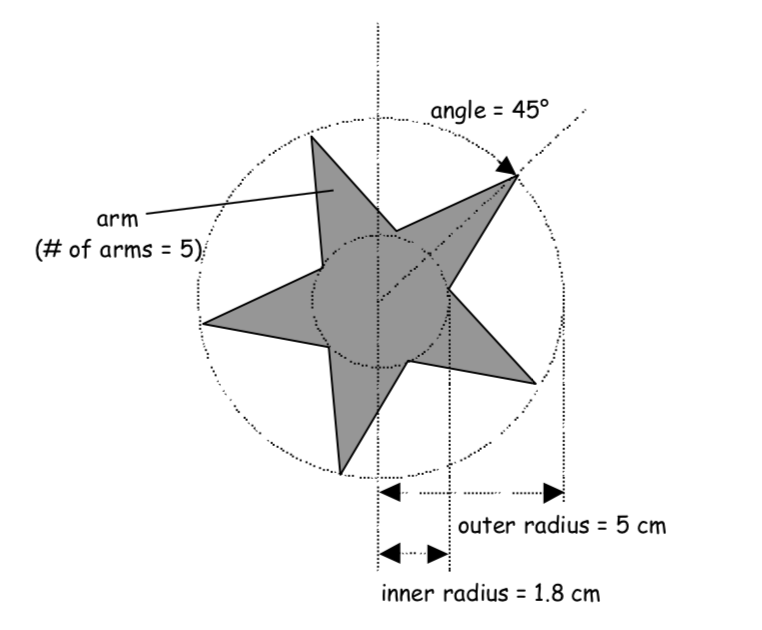
\includegraphics[width=13cm]{images/star_features}
	\caption{Koncept hvězdy (Figure 52 z \cite{Czarnecki98} )}
\end{figure}

\subsection{Kompozice}
V kompozičním modelu spojíme několik komponent dohromady, které tak vytvoří požadovaný celek. K tomu, abychom byli schopni generovat různé hvězdy, je potřeba mít sadu konkrétních komponent různých velikostí a tvarů.
\begin{figure}[H]
	\centering
	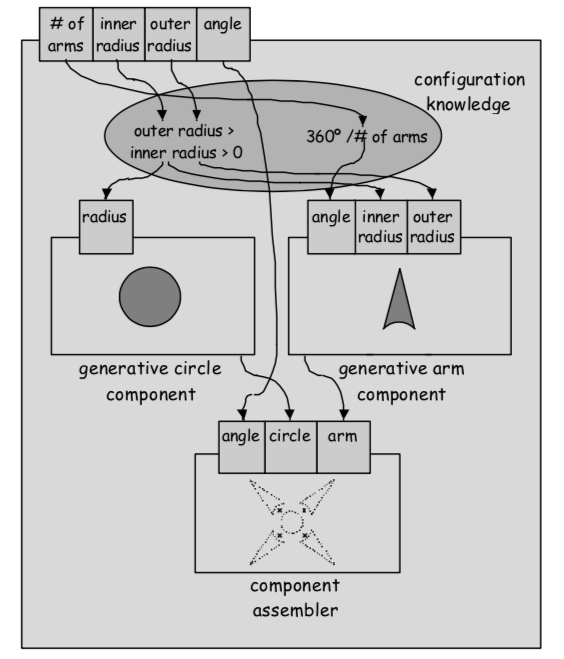
\includegraphics[width=13cm]{images/generating_process}
	\caption{Proces generování hvězdy (Figure 55 z \cite{Czarnecki98} )}
\end{figure}
Kruh je popsán pouze vnitřním poloměrem, zatímco cípy jsou popsány vnitřním poloměrem, jejich počtem a vnějším poloměrem. K tomu abychom sestavili čtyřcípou hvězdu, která je vidět na obrázku, je potřeba jeden kruh a čtyři cípy vybrané ze sady konkrétních komponent, na základě jejich vlastností.
\begin{figure}[H]
	\centering
	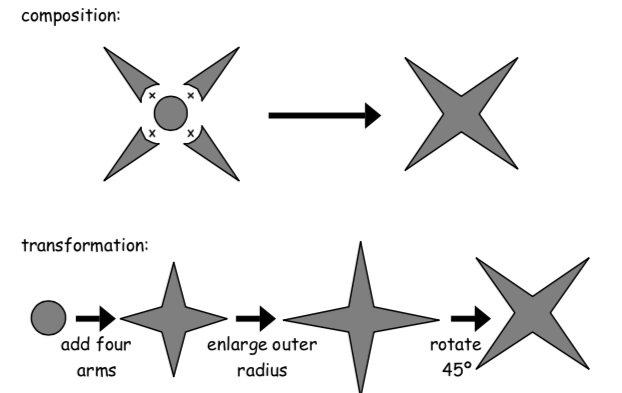
\includegraphics[width=13cm]{images/comparison}
	\caption{Sestavení hvězdy pomocí kompozice nebo transformace (Figure 53 z \cite{Czarnecki98} )}
\end{figure}
Efektivnějším způsobem sestavení instance je použití \textit{generativních komponent} místo konkrétních komponent. Generativní komponenta využívá abstraktního popisu komponent a generuje komponentu na základě popisu. Například místo celé sady všech možných kruhů a cípů potřebujeme dvě generativní komponenty, a to generativní kruh a generativní cíp. Generativní kruh má jako parametr vnitřní poloměr a generativní cíp má jako své parametry vnitřní poloměr, vnější poloměr a úhel.
\begin{figure}[H]
	\centering
	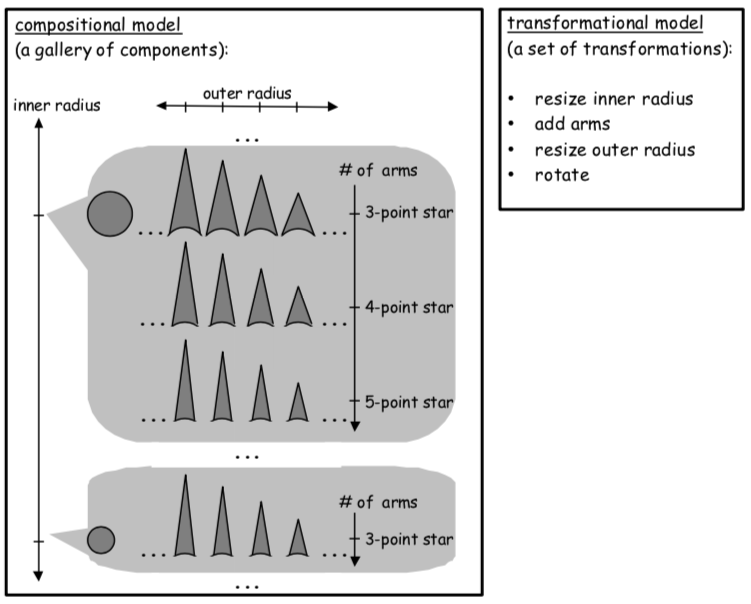
\includegraphics[width=13cm]{images/transformation_vs_composition}
	\caption{Doménový model hvězdy pomocí kompozice (vlevo) nebo transformace (vpravo) (Figure 54 z \cite{Czarnecki98} )}
\end{figure}
Konkrétní komponenty jsou následně vygenerovány a poskládány do požadovaného obrazce.

\subsection{Transformace}
Narozdíl od kompozice nespojujeme jednotlivé komponenty, ale provádíme určitý počet transformací, které vyústí v požadovaný výsledek. Není potřeba mít nadefinovanou sadu komponent, nebo jejich generování, ale je třeba mít nadefinované transformace, které můžeme s instancí provádět. V tomto příkladě jsou to transformace: 
\begin{itemize}
	\item přidej 4 cípy
	\item zvětš vnější poloměr
	\item otoč o 45 stupňů
\end{itemize}

\subsection{Aplikace na software}
V minulých částech bylo popsáno, jakými způsoby jsou tvořeny generátory. Generátory se však používají především v softwarovém odvětví. Příklad, na kterém bude generátor demonstrován, bude editor GUI.

Součástí programátorského prostředí Visual Studio od společnosti Microsoft je tvorba aplikací pro windows, nebo-li \textit{Windows Form Application}. Součástí těchto aplikací je grafické uživatelské prostředí (\textit{GUI}). GUI je stejně jako logika aplikace popsáno zdrojovým kódem. Tento kód je ale možné generovat přes editor GUI. Po otevření editoru je programátorovi nabídnuto okno výchozí velikosti. Dále je mu nabídnut kontejner, který obsahuje veškeré komponenty, které se v tomto druhu aplikací objevují. Obsahuje například tlačítka (z angl. \textit{button}), textová pole (z angl. \textit{textBox}) a mnoho dalších. Programátor vybírá komponenty z kontejneru a umišťuje je do okna, podle potřeby. Každá komponenta má vícero vlastností. Těmito vlastnostmi jsou například umíštění, text a další.

Během umišťování komponent do okna je Visual Studiem generován kód, který tyto komponenty popisuje. Programátor typicky do tohoto kódu následně dopisuje požadované reakce na různá tlačítka, obsahy různých listů a mnoho dalšího. Tento výsledný kód je následně součástí aplikace. 


\begin{figure}[H]
	\centering
	\makebox[\linewidth]{
		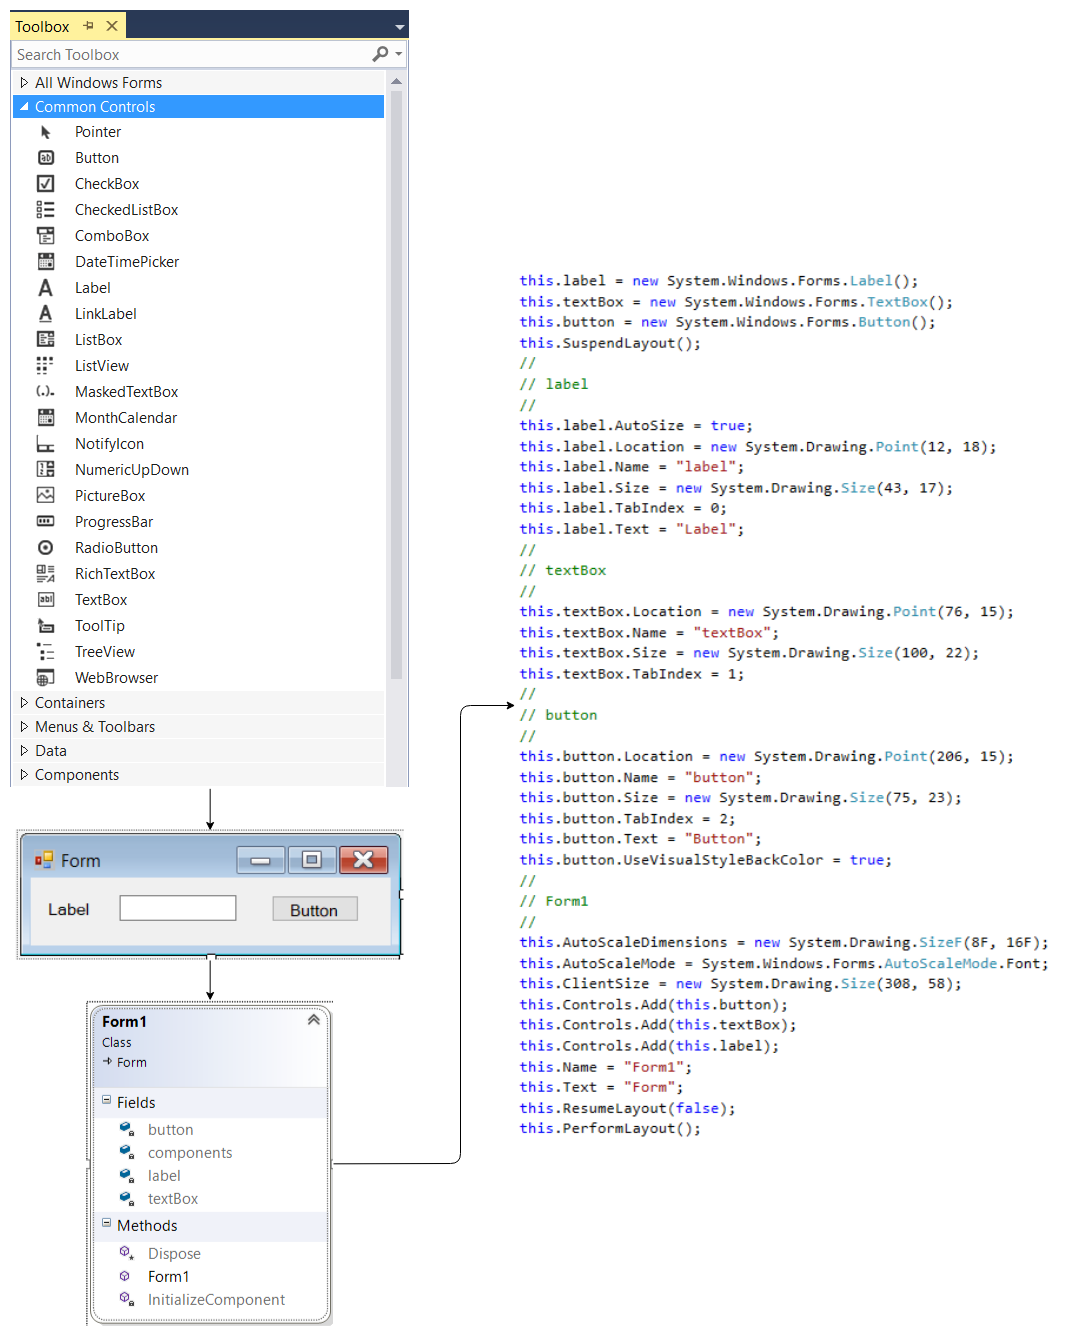
\includegraphics[width=1.25\linewidth]{images/diagram}
	}
	\caption{Proces generování}
\end{figure}

Tento přístup k tvorbě GUI šetří programátorovi spoustu času, který by bez editoru musel vynaložit na napsání kódu celého uživatelského rozhraní.

\section{Shrnutí}
I když se transformační generátor zdá být jednodušśí, většina generátorů, které známe, jsou kompoziční. Příkladem takového generátoru může být editor GUI, který na základě grafického editoru, ve kterém poskládáme grafické komponenty dohromady, vygeneruje kód, který je popisuje, jak je vidět na obrázku 4.5.

Kompoziční generátor bude použit v této práci. Na základě vytvořené varianty z modelu vlastností bude generován kód jazyka tesa. Komponenty zde budou zaznamenány jako záznamy v souboru formátu XML. Z těchto komponent bude následně vygenerován výsledný kód.


